\section{Genetic Algorithm}
	Genetic algorithms are a population based heuristic method that simulates nature's evolutionary system to evolve a starting population of random solutions to obtain very good (possibly optimal) solutions at the end of the process. To do this a random starting population is generated, then each solution is evaluated with a fitness function. After that some solutions, usually the best ones, are chosen to create offsprings that will replace worst solutions. This way the algorithm performs a sort of natural selection keeping the best solutions and improving them over generations.
	
	As the problem is a variation of the popular Traveling Salesman Problem (TSP), it will be traded as such, so operators and solution representation are often the one used in literature for that problem. Also the important thing in the solution is the order of visited nodes, so crossover and mutations are order preserving, this means that they don't generate many new connections but try te keep connected the nodes that were already connected before.
		
	\subsection{Encoding}
		To represent a TSP solution the path representation has been used, it consists in a sequence of $N$ nodes, where $N$ is the total number of nodes, sorted from the starting one to the last visited on encoded path.
		
		For example the path $0 \rightarrow 3 \rightarrow 1 \rightarrow 4 \rightarrow 2 \rightarrow 0$ is encoded as:
		\[[0, 3, 1, 4, 2]\]
		Note that there are some symmetries using this representation:
		\begin{enumerate}
			\item \textit{Rotation symmetries}: By rotating the path we obtain a solution that is equivalent but simply starts from a different node, e. g. [0,3,1,4,2] and [3,1,4,2,0]. These have been removed by fixing starting node to 0.
			\item \textit{Direction symmetry}: By reversing all the elements but the first of a path we get a representation of the inverse path, e.g. [0,3,1,4,2] and [0,2,4,1,3]. Dealing with this symmetry is however not efficient and so it's not been removed.
		\end{enumerate}
	
	\subsection{Fitness}
		As fitness concerns I took a different approach from usual genetic algorithms and considered the sum of costs in path as the fitness and I will try to minimize it.
		This choice was taken because other considered fitness functions had drawbacks, mainly because most of them were in the form $upperBound - costs$ but upper bounds are not so strict and then a proportional choice based on fitness would yield a very similar probability for each individual (because $maxFitness - minFitness$ is much lower than $upperBound - anyFitness$).
		
		By setting the fitness function equal to the sum of path costs it it directly proportional to objective function resulting in a more correct reward based on fitness.
		
	\subsection{Select}
		The select operator is a little tricky because of the fact that solutions with lower fitness should have higher probabilities, so both Montecarlo and Linear ranking methods can't be used. N-Tournament is a valid alternative, but it was discarded because if a subset of $k$ solutions is chosen, the $k-1$ worst solutions are never used for crossover and this reduces (slightly) diversification.
		
		The final choice is a probability calculated based on position in an array of solutions sorted by fitness. The selected solution is the one with index
		\[index = \left \lfloor{N * r^{2}}\right \rfloor\]
		where N is the total number of nodes and r is a random number $\in [0, 1)$
		
		This way the solutions with lower cost are more likely to be chosen than the others, but each solution might be selected.
		
	\subsection{Crossover}
		The crossover operator takes a certain number of parents and creates an offspring that inherits parents properties. In the project was used the Order Crossover (OX), that from 2 parents creates one child, and works like this:
		
		\begin{figure}[h]
		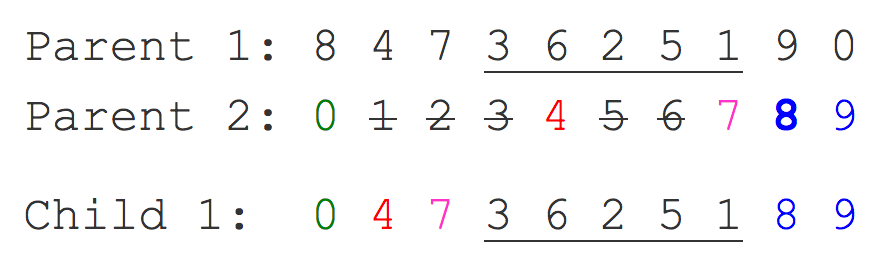
\includegraphics[width=0.6\textwidth]{ox_crossover}
		\centering
		\caption{Example of Order Crossover (OX)}
		\end{figure}
		
		\begin{enumerate}
			\item Select a random subsequence of consecutive alleles from parent 1. (underlined)
			\item Drop the subsequence down to Child and mark out these alleles in Parent 2.
			\item Starting on the right side of the subsequence, grab alleles from parent 2 and insert them in Child at the right edge of the subsequence. Since 8 is in that position in Parent 2, it is inserted into Child first at the right edge of the subsequence.\\
				Notice that alleles 1, 2 and 3 are skipped because they are marked out and 4 is inserted into the 2nd spot in Child.
		\end{enumerate}
		
	\subsection{Mutation}
		Only one type of mutation is used and it is the 2-opt, an algorithm that takes a substring of the path representation and reverse it. The idea is to take a route that crosses over itself and reorder it so that it does not.
		This is good for the main purpose of mutations (prevent genetic drift) as well as for improving solutions.
		
		\begin{figure}[h]
		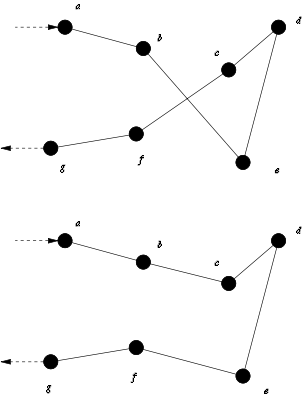
\includegraphics[width=0.5\textwidth]{2-opt}
		\centering
		\caption{Example of 2-opt mutation}
		\end{figure}
		
		To control the mutation there is a parameter MUTATION\_CHANCE that sets the probability that this mutation happens.
		
	\subsection{Generational Replacement}
		When a population advance to next generation we need to replace the old bad solutions with newly created offsprings. This is done by elitist, so only the best solutions are kept and all the others are replaced by new solutions. The percentage of survivors (and replaced solutions) is set by the parameter SURVIVAL\_RATIO.
		
	\subsection{Improvements}
		After implementing all the elements of the algorithm and doing some basic tests I found out that the convergence was fast and after a few generations the solution was already quite good and it was rarely improved after. This means that algorithm was iterating through a lot of generation with very few improving solutions, so I decided to introduce random restarts reducing generations count and considering the best solution from all evaluated populations. This approach worked out well to find more reliably good solutions but slowed computation down. To make up for the loss in performance multithread has been used running genetic algorithm on many random starting populations in parallel. It is possible to control the amount of populations evaluated by setting the parameter POPULATIONS.
		
		Another thing that has been tested is to modify the mutation chance at runtime based on the number of non-improving generations, but this didn't lead to significative improvement of solutions.
		
		